\documentclass[uplatex]{jsarticle}
\usepackage{octopus}
\usepackage{url}

% \newtheorem{teiri}{定理}[section]
% \newtheorem{teigi}[theo]{定義}
% \newtheorem{hodai}[theo]{補題}
% \newtheorem{prop}[theo]{命題} % 以下は再定義の必要はない
% \newtheorem{corr}[theo]{系}
% \newtheorem{rei}[theo]{例}

\renewcommand{\proofname}{\textsf{証明}}
\renewcommand{\postpartname}{章}
\renewcommand{\thesection}{\thepart.\arabic{section}}
\renewcommand{\thepart}{\arabic{part}}
\makeatletter\renewcommand{\theequation}{\thesection.\arabic{equation}}\@addtoreset{equation}{section}\makeatother

\newcommand{\octopuspart}[1]{\newpage\part{#1}\setcounter{section}{0}\vspace{3\baselineskip}}

\DeclareMathOperator{\dcup}{\dot{\cup}}


% イントロダクション+距離空間 [ノート]
% 位相空間: 定義と例 [ノート]
% 位相空間: 連結性 [ノート]
% 位相空間: コンパクト性 [ノート]
% 位相幾何: ホモトピー [ノート]
% 位相幾何: 基本群 [ノート]
% 位相幾何: 被覆空間 [ノート]
% 位相幾何: ホモロジー [ノート]
% 位相幾何: ホモロジーの計算 [ノート]
% 位相幾何: 特異ホモロジー [ノート]
% テンソル: 双対空間,テンソルの定義 [ノート]
% テンソル: 反変ベクトル,共変ベクトル,スカラー,混合テンソル [ノート]
% テンソル: 交代テンソル,擬テンソル,テンソル密度,Eddintonのε [ノート]

\begin{document}
\begin{center}{\LARGE \bf 幾何数理工学 ノート}\end{center}

\midashi{本講義の内容}
\begin{enumerate}
    \item 位相空間:「近さ」が備わった空間概念。$\mathbb{R}^{n}$の一般化。
    \item 位相幾何:連続変形に対する不変性。
    \begin{itemize}
        \item 基本群
        \item ホモロジー
    \end{itemize}
    \item テンソル:座標変換に対する不変性。
    \begin{itemize}
        \item 3次元ベクトル${\displaystyle \begin{pmatrix}
            v_{1} & v_{2} & v_{3} 
        \end{pmatrix}^{\top}}$と${\displaystyle \begin{pmatrix}
            \pdif{f}{x_{1}} & \pdif{f}{x_{2}} & \pdif{f}{x_{3}}
        \end{pmatrix}^{\top}}$の違いは何か。
    \end{itemize}
\end{enumerate}

\midashi{参考書}
\begin{itemize}
    \item 内田伏一,「集合と位相」\footnote{amazonだと2,808円。}
    \item Allen Hatcher,「Algebraic Topology」\footnote{\url{https://pi.math.cornell.edu/~hatcher/AT/ATpage.html}}
    \item 伊理正夫,韓太舜,「テンソル解析入門」\footnote{楽天だと2,097円(税)。}
\end{itemize}

\renewcommand{\baselinestretch}{0.1}
\tableofcontents
\renewcommand{\baselinestretch}{1.0}

\octopuspart{位相空間}
\section{距離空間}

\begin{teigi}
    $X$を非空な集合,$d: \, X \times X \to \mathbb{R}$を実数値関数とする。次の三つの条件{\bf D1},{\bf D2},{\bf D3}を考える。
    
    \midashi{D1. } $\forall x, y \in X, \quad d(x,y) \ge 0$,\qquad $d(x,y) = 0 \quad \Longleftrightarrow \quad x = y$
    
    \midashi{D2. } $\forall x, y \in X, \quad d(x,y) = d(y,x)$
    
    \midashi{D3. } $\forall x, y \in X, \quad d(x,y) + d(y,z) \ge d(x,z)$
    
    $d$が{\bf D1},{\bf D2},{\bf D3}の条件を満たすとき,$d$を$X$上の\nw{距離関数}という。

    また,$X$あるいは$(X,d)$を\nw{距離空間}(metric space)という。
\end{teigi}

{\bf D2.}は対称性を表し,{\bf D3.}は三角不等式と呼ばれる。

{\bf D1.},{\bf D2.},{\bf D3.}を満たさないような関数として,例えば${d_{2}}^{2}$(2乗距離)がある。
これは三角不等式を満たさない。

\begin{rei}
    $X = \mathbb{R}^{n}$とする。
    \begin{align}
        d_{2} (x,y) &:= \sqrt{\sum_{i=1}^{n} (x_{i} - y_{i})^{2}}, \\
        d_{1} (x,y) &:= \sum_{i=1}^{n} |x_{i} - y_{i}|, \\
        d_{\infty} (x,y) &:= \max_{i} |x_{i} - y_{i}|
    \end{align}
    とすると,これらはどれも$X$上の距離関数である。なお,$(\mathbb{R}^{n}, d_{2})$を\nw{$n$次元Euclid空間}と呼ぶ。
\end{rei}
\begin{proof}
    ここでは$d_{2}$が{\bf D3.}の三角不等式を満たすことのみを示す。
    \begin{align}
        {d_{2}}^{2}(x,z)
        &= \sum_{i=1}^{n} (x_{i} - z_{i})^{2} = \sum_{i=1}^{n} (x_{i} - y_{i} + y_{i} - z_{i})^{2} \notag \\
        &= \sum_{i=1}^{n} \left( x_{i} - y_{i} \right)^{2} + \sum_{i=1}^{n} \left( y_{i} - z_{i} \right)^{2} + 2 \sum_{i=1}^{n} \left( x_{i} - y_{i} \right) \left( y_{i} - z_{i} \right) \notag \\
      &\le \sum_{i=1}^{n} \left( x_{i} - y_{i} \right)^{2} + \sum_{i=1}^{n} \left( y_{i} - z_{i} \right)^{2} + 2 \sqrt{\left( \sum_{i=1}^{n} \left( x_{i} - y_{i} \right)^{2} \right) \left( \sum_{i=1}^{n} \left( y_{i} - z_{i} \right)^{2} \right)} \label{eq:1.1:Cauchy}\\
        &= \left\{ \sqrt{\sum_{i=1}^{n} \left( x_{i} - y_{i} \right)^{2}} + \sqrt{\sum_{i=1}^{n} \left( y_{i} - z_{i} \right)^{2}} \right\}^{2}
         = \left( d_{2}(x,y) + d_{2} (y,z) \right)^{2}
    \end{align}
    である。ここで,式\eqref{eq:1.1:Cauchy}に至る変形にはCauchy-Schwarzの不等式が用いられている。
\end{proof}

\begin{rei}
    $X = \mathcal{C} [a,b]$を区間$[a,b] \subseteq \mathbb{R}$上の連続関数全体の集合とする。
    \begin{align}
        d_{2} (f,g) &:= \sqrt{ \int_{a}^{b} | f(t) - g(t) | ^{2} \dx{t}}, \\
        d_{\infty} (f,g) &:= \sup \sets{ \left| f(t) - g(t) \right| | t \in [a,b]}, \\
        d_{1} (f,g) &:= \int_{a}^{b} \left| f(t) - g(t) \right| \dx{t}
    \end{align}
    とすると,これらはどれも$X$上の距離関数である。
\end{rei}

\begin{proof}
    ここでは$d_{1}$が{\bf D3.}の三角不等式を満たすことと{\bf D1.}の零点が対角集合に限られることのみを示す。

    \midashi{{\bf D3.}について}
    \begin{align*}
        d_{1} (f,h)
        &= \int_{a}^{b} \left| f(t) - h(t) \right| \dx{t} \\
      &\le \int_{a}^{b} \left( \left| f(t) - g(t) \right| + \left| g(t) - h(t) \right| \right) \dx{t} \\
      &\le \int_{a}^{b} \left| f(t) - g(t) \right| \dx{t} +  \int_{a}^{b} \left| g(t) - h(t) \right| \dx{t} \\
        &= d_{1} (f,g) + d_{1} (g,h)
    \end{align*}
    で従う。

    \midashi{零点が対角集合に限られることについて}

    $f = g$ならば$d_{1} (f,g) = 0$は明らかであるので,問題はその逆である。

    もし,$f(x) \neq g(x)$ならばある$x_{0} \in [a,b]$で$\left| f(x_{0}) - g(x_{0}) \right|> 0$であり,
    $f-g$の連続性からある$\varepsilon > 0$が存在して,$y \in [x_{0} - \varepsilon, x_{0} + \varepsilon]$に対して
    $\left| f(y) - g(y) \right| > 0$である。
    したがって,
    \begin{equation*}
        \int_{a}^{b} \left| f(x) - g(x) \right| \dx{x} \ge \varepsilon \min_{x_{0} - \varepsilon \le y \le x_{0} + \varepsilon} \left| f(y) - g(y) \right| > 0
    \end{equation*}
    である。
\end{proof}

\begin{rei}
    $X = \sets{0,1}^{n}$とする。
    \begin{equation}
        d_{H}(x,y) = \# \sets{i | x_{i} \neq y_{i}}
    \end{equation}
    で定めると,これは$X$上の距離関数である。この距離関数は\nw{Hamming距離}と呼ばれる。
\end{rei}

%%% 綴り

\begin{rei}
    $G = (X,E)$を無向グラフとする。
    $d_{G}(x,y)$を$x$から$y$への最短路の長さとして定義すると,
    これは$G$上の距離関数である。
\end{rei}

以下,$(X,d)$を距離空間とする。

\begin{teigi} %閉包まで
    \midashi{1. } $a \in X$,$\varepsilon > 0$とする。集合$N(a,\varepsilon) := \sets{x \in X | d(a,x) < \varepsilon}$を,$a$の\nw{$\varepsilon$-近傍}という。

    \midashi{2. } $A \subseteq X$の\nw{内点}とは,次の条件を満たす点$x \in X$のこと:
    \begin{equation}
        \exists \varepsilon > 0, \quad N(x,\varepsilon) \subseteq A
    \end{equation}
    また,$A$の内点全体の集合$A^{\circ} = \sets{x \in X | N(x, \varepsilon) \subseteq A}$のことを$A$の\nw{内部}という。

    \midashi{3. } $A \subseteq X$の\nw{外点}とは,次の条件を満たす点$x \in X$のこと:
    \begin{equation}
        \exists \varepsilon > 0, \quad N(x , \varepsilon ) \cap A = \emptyset
    \end{equation}
    言い換えると,$A$の補集合の内点のこと。
    また,$A$の外点全体の集合$(X \setminus A)^{\circ}$を$A$の\nw{外部}という。

    \midashi{4. } $A \subseteq X$の\nw{境界点}とは,次の条件を満たす点$x \in X$のこと:
    \begin{equation}
        \forall \varepsilon > 0, \quad N(x, \varepsilon) \cap A \neq \emptyset, \, N(x,\varepsilon) \cap (X \setminus A) \neq \emptyset
    \end{equation}
    また,$A$の境界点全体の集合のことを$A$の\nw{境界}といい,記号$\partial A$で表す。

    \midashi{5.} $A \subseteq X$の\nw{触点}とは,次の条件を満たす点$x \in X$のこと:
    \begin{equation}
        \forall \varepsilon > 0, \quad N (x,\varepsilon) \cap A \neq \emptyset
    \end{equation}
    また,$A$の触点全体の集合のことを$A$の\nw{閉包}といい,記号$\overline{A}$で表す。
\end{teigi}

\begin{figure}[htbp]
    \centering
    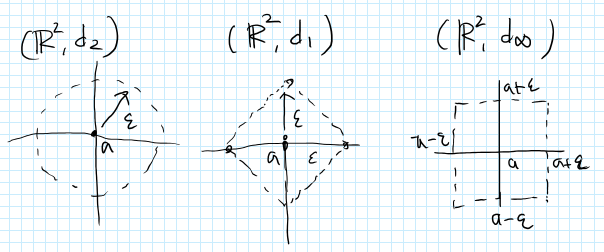
\includegraphics[clip,width=0.8\columnwidth]{euclid_dist.png}
    \caption{距離空間$(\mathbb{R}^{2},d)$上の近傍の違い}
    \label{fig:euclid_dist}
\end{figure}

\begin{figure}[htbp]
    \centering
    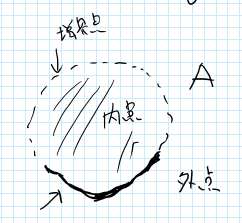
\includegraphics[clip,width=0.3\columnwidth]{in_ex_boundary.png}
    \caption{$A \subseteq X$の内部,外部,境界}
    \label{fig:in_ex_boundary}
\end{figure}

この定義から,内部,外部,境界点について
\begin{equation}
    X = A^{\circ} \dcup \partial A \dcup (X \setminus A)^{\circ}
\end{equation}
と互いに非交な集合に分解できる。
また,閉包について,次の二つが成り立つ。
\begin{align}
    & A ^ { \circ } \subseteq A \subseteq \overline { A } \\
    & \overline { A } = A ^ { \circ } \cup \partial A
\end{align}

\begin{teigi}
    \begin{equation*}
        \begin{array}{lcccl}
            A \subseteq X \text{:\nw{開集合}} & \defines & \forall x \in A, \quad \exists \varepsilon > 0, \quad  N(x , \varepsilon ) \subseteq A & \Longleftrightarrow & A = A^{\circ} \\
            A \subseteq X \text{:\nw{閉集合}} & \defines & 「\forall x \in X, \quad \forall \varepsilon > 0, \quad  N(x , \varepsilon ) \cap A \neq \emptyset \Longrightarrow x \in A」& \Longleftrightarrow & A = \overline{A} \\
        \end{array}
    \end{equation*}
\end{teigi}

\begin{hodai}
    $N(x,\varepsilon)$は開集合。特に,$N(x,\varepsilon) = N(x,\varepsilon)^{\circ}$。
\end{hodai}

\begin{proof}
    $y \in N ( x, \varepsilon)$をとる。$\delta := \varepsilon - d ( x , y ) > 0$とすると,
    $z \in N(y, \varepsilon)$に対して,三角不等式より
    \begin{equation}
        d(x,z) \le d(x,y) + d(y,z) < \varepsilon
    \end{equation}
である。よって,$N(y,\delta) \subseteq N(x,\varepsilon)$となる。
\end{proof}

\begin{prop}
    $\left( A^{\circ} \right)^{\circ} = A^{\circ}$,$\overline{\overline{A}} = \overline{A}$
\end{prop}

\begin{proof}
    $\left( A^{\circ} \right)^{\circ} \subseteq A^{\circ}$より,$\supseteq$向きを示す。
\end{proof}

\begin{prop}
    \midashi{1. } $A$:開 $\Longrightarrow$ $X \setminus A$:閉

    \midashi{2. } $A$:閉 $\Longrightarrow$ $X \setminus A$:開
\end{prop}

\begin{proof}
    
\end{proof}

開集合全体の集合を\nw{開集合系}といい,記号$\mathcal{O}$で表す。
閉集合全体の集合を\nw{閉集合系}といい,記号$\mathfrak{A}$で表す。

\begin{prop}
    \label{prop:open_set_axiom}
    開集合系$\mathcal{O}$について以下が成り立つ。

    \midashi{1. } $X \in \mathcal{O}$,$\emptyset \in \mathcal{O}$

    \midashi{2. } $O_{1}, O_{2}, \cdots, O_{k} \in \mathcal{O} \Longrightarrow O_{1} \cap O_{2} \cap \cdots \cap O_{k} \in \mathcal{O}$

    \midashi{3. } 任意の集合$\Lambda$に対して$O_{\lambda} \in \mathcal{O}$($\forall \lambda \in \Lambda$) ${\displaystyle \Longrightarrow \bigcup_{\lambda \in \Lambda} O_{\lambda} \in \mathcal{O}}$
\end{prop}

\begin{proof}
    \midashi{1. } obvious.

    \midashi{2. }

    \midashi{3. }
\end{proof}

\begin{prop}
    閉集合系$\mathfrak{A}$について以下が成り立つ。
    
    \midashi{1. } $X \in \mathfrak{A}$,$\emptyset \in \mathfrak{A}$

    \midashi{2. } $A_{1}, A_{2}, \cdots, A_{k} \in \mathfrak{A} \Longrightarrow A_{1} \cup A_{2} \cup \cdots \cup A_{k} \in \mathfrak{A}$

    \midashi{3. } 任意の集合$\Lambda$に対して$A_{\lambda} \in \mathfrak{A}$($\forall \lambda \in \Lambda$) ${\displaystyle \Longrightarrow \bigcap_{\lambda \in \Lambda} A_{\lambda} \in \mathfrak{A}}$
\end{prop}

\begin{proof}
    \midashi{1. } $\mathfrak{A} = \sets{ X \setminus O | O \in \mathcal{O}}$に注意すると明らか。

    \midashi{2. }

    \midashi{3. }
\end{proof}

収束性,連続性なども距離空間で定義できる。

\begin{teigi}
    \midashi{1. } $a_{i} \in X$($i=1,2,\dots$):\nw{収束}とは,
    \begin{equation}
        \lim_{i \to \infty} a_{i} = a \defines \lim_{i \to \infty} d(a, a_{i}) = 0
    \end{equation}
    
    \midashi{2. } $f:X \longrightarrow \mathbb{R}$が$a \in X$で\nw{連続}とは,
    \begin{equation}
        \forall \varepsilon > 0, \quad \exists \delta > 0, d(a,x) < \delta \Longrightarrow \left| f(a) - f(x) \right| < \varepsilon
    \end{equation}
\end{teigi}
\section{位相空間}
\section{連結性}
\section{コンパクト性}

\octopuspart{位相幾何}
連続変形に対する不変性

\section{ホモトピー}
\section{基本群}
\section{被覆空間}
\section{ホモロジー}
\section{ホモロジーの計算}
\section{特異ホモロジー}

\octopuspart{テンソル}
座標変換に対する不変性

\section{双対空間}
\section{テンソルの定義}
\section{反変性・共変性・スカラー・混合テンソル}
\section{交代テンソル・擬テンソル・テンソル密度・Eddintonのε}


\begin{teigi}
    fff
\end{teigi}

\begin{teiri}
    \midashi{(1)}fff
\end{teiri}

\begin{hodai}
    \midashi{(1)}
\end{hodai}

\begin{rei}
    fdd
\end{rei}
bibifdd
\end{document}